% =====================================================================================
% Starter manuscript. On the first Overleaf sync:
%   - blank Overleaf project      -> this file goes to Overleaf;
%   - Overleaf already has a draft -> the draft replaces this file (and references.bib).
%
% Journal class: replace the \documentclass line, for example
%   APS (PRA, PRL, ...): \documentclass[aps,pra,twocolumn,superscriptaddress,10pt]{revtex4-2}
%                        (put \maketitle after the abstract, use \affiliation, drop \date)
%   Elsevier:            \documentclass[preprint,12pt]{elsarticle}
%   Springer Nature:     use the sn-jnl template from the journal's Overleaf page
% =====================================================================================
\documentclass[11pt]{article}

\usepackage[margin=2.5cm]{geometry}
\usepackage{graphicx}
\usepackage{amsmath,amssymb}
\usepackage{bm}
\usepackage{booktabs}
\usepackage{xcolor}
\usepackage[numbers,sort&compress]{natbib}
\usepackage{hyperref}

\hypersetup{colorlinks=true, linkcolor=blue!50!black, citecolor=blue!50!black, urlcolor=blue!50!black}
\graphicspath{{figures/}}              % figures written by run/*.py land in paper/figures/

% Working notes: \showtodostrue -> \showtodosfalse hides every \TODO
\newif\ifshowtodos \showtodostrue
\newcommand{\TODO}[1]{\ifshowtodos\textcolor{red}{\textbf{[TODO:} #1\textbf{]}}\fi}

\title{\TODO{Title of the paper}}
\author{Gubio G. de Lima\thanks{\TODO{affiliation}. E-mail: \texttt{gubio.gomes@estudante.ufscar.br}}}
\date{\today}

\begin{document}
\maketitle

\begin{abstract}
\TODO{Abstract -- write it last.}
\end{abstract}

\section{Introduction}\label{sec:intro}
\TODO{Context, gap, contribution, outline.} Citations come from \texttt{references.bib}, for
example~\cite{example2024}.

\section{Methods}\label{sec:methods}
\TODO{Model, data and procedure.}

\section{Results}\label{sec:results}
Figure~\ref{fig:example} is produced by \texttt{run/example\_figure.py}, which writes it directly into
\texttt{paper/figures/}; a new run followed by a push updates it here and in Overleaf.

\begin{figure}[t]
  \centering
  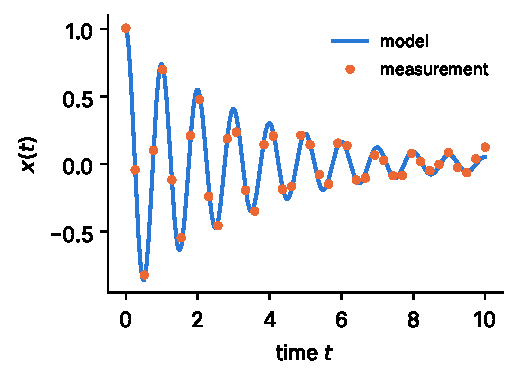
\includegraphics[width=0.6\linewidth]{example.pdf}
  \caption{Example figure: damped oscillation (line) and noisy measurements (points).}
  \label{fig:example}
\end{figure}

\section{Conclusions}\label{sec:conclusions}
\TODO{}

\bibliographystyle{unsrtnat}
\bibliography{references}

\end{document}
